\subsection{Prediction Evaluation}

\subsection{Weather Data}
\label{sec:experiments-weather}

The example below shows our model generated on monthly rainfall and temperature data
collected over the course of 20 years between 1920 and 1940 in Nottingham England.

\begin{figure}[h!]
	\centering
	\makebox[\textwidth]{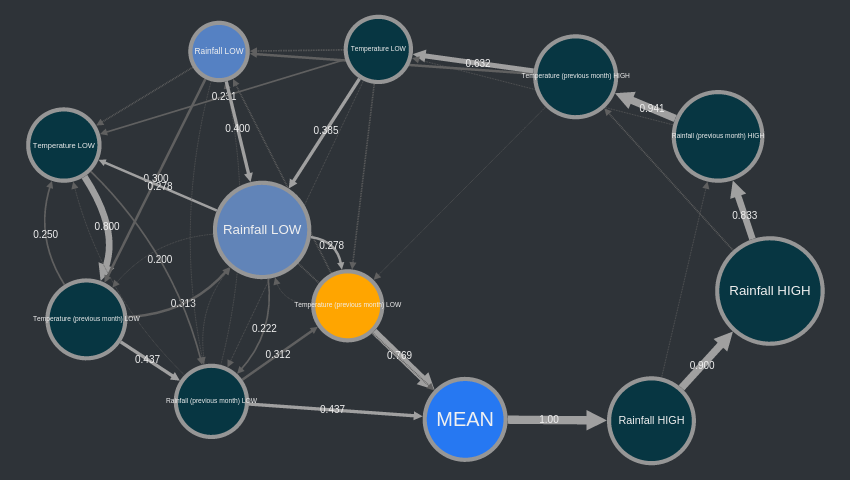
\includegraphics[width=100pt]{example-weather}}
	\caption{Qualitative representation of temperature and rainfall data collected over the course of 20 years.}
	\label{fig:example-weather}
\end{figure}

\subsection{GPS Data}

\subsection{Domain Experts}